\chapter{Résoudre un Rubik's cube}

\section{Le besoin}
Cette partie est le coeur du projet: il s'agit de créer un algorithme étant capable d'à partir d'un Rubik's Cube quelconque, de trouver la suite des rotations pour le résoudre. Celui-ci doit être le plus rapide possible, tant en terme de temps d'exécution qu'en terme de complexité de la solution trouvée, c'est à dire le nombre de rotations qui seront effectuées pour résoudre le cube.

\section{Modéliser un Rubik's Cube}

Dans ce projet, nous nous sommes rendu compte que modéliser un Rubik's Cube était moins trivial qu'il n'en avait l'air.
Le modèle qu'on cherchait devait respecter plusieurs critères. 
\begin{enumerate}
    \item Premièrement nous devions avoir une interface pour récupérer la couleur de chaque facette à tout moment.
    \item Ensuite il fallait qu'on ait une fonction qui simule une rotation sur une couronne quelconque.
    \item Enfin, notre modélisation devait être assez efficace pour permettre une résolution qui ne prenne pas trop de temps.
\end{enumerate}
\subsection{Les premières idées naïves}

\subsubsection{Le tableau de facettes}
La première idée qui nous est venue est de stocker la couleur de chaque facette dans un tableau.
Cette méthode n'est pas très efficace: créer une fonction pour simuler la rotation d'une couronne s'avère être compliqué.
De plus la complexité en mémoire n'est pas très bonne.

\subsubsection{La liste chaînée}
Similairement à cette première méthode, nous avons également songé à stocker les couleurs dans une liste chaînée en 2 dimensions.
On aurait "mis à plat" le Rubik's Cube et on aurait parcouru ses facettes sur un plan infini.

\subsubsection{Les cubies}
La deuxième idée que nous avons eu était de considérer les \textit{cubies}, petits cube constituant le Rubik's Cube en 3x3x3.
La rotation semblait être plus facile car nous aurions pu travailler avec des transformations d'angles et de position dans l'espace.
Cependant cette méthode faisait apparaître des complications d'implémentations rendant notre code très lourd.

\subsection{Le tableau de permutations}
Nous avons finalement décidé d'adopter une approche plus mathématique : le tableau de permutations.

Cela consiste en un tableau de 6*8=48 cases (six faces et 8 facettes qui peuvent bouger).
Le Rubik's résolu est alors représenté par un tableau rempli de 0 à 47 (dans l'ordre).
Effectuer une rotation est alors équivalent à appliquer une permutation sur le tableau.
Cela s'implémente simplement et l'algorithme est efficace.
Retrouver la couleur en fonction du numéro dans la case du tableau est aisé en définissant les permutations.

\begin{figure}[h]
\begin{center}
    \makebox[\textwidth]{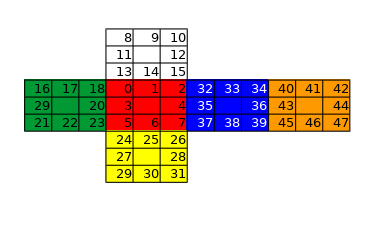
\includegraphics[width=.5\paperwidth]{diagrammes/perm.png}}
\end{center}
    \caption{Les permutations du Rubik's}
\end{figure}

C'est finalement cette approche que nous avons décidé de garder car elle nous permettait de garder un code simple et efficace.

\section{Algorithme de résolution}
Une fois que nous avons créé un objet représentant le cube que nous pouvions manipuler virtuellement, nous nous sommes attaqué à la partie résolution.
Résoudre un Rubik's Cube nécessite d'être rigoureux et surtout méthodique.
C'est donc pourquoi nous avions initialement pensé qu'un ordinateur serait parfaitement adapté pour appliquer une méthode de résolution.
Cependant, nous nous sommes aperçu que il y a toujours une partie d'intuition dans les méthodes de résolution (par exemple faire la première face).
Cela nous a donc posé une difficulté.

\subsection{Les premiers essais}
Le premier essai a été d'adapter la méthode de résolution qu'un humain met en place lorsqu'il apprend à résoudre le cube. Cette méthode se repose sur des manoeuvres connues qui doivent être exécutées dans un certain ordre prédéterminé.
Ces manoeuvres doivent êtres exécutées lorsqu'on détecte une certaine configuration, c'est à dire lorsque la configuration du cube correspond à l'une des configurations dans laquelle la manoeuvre peut être exécutée. Cette approche devait par ailleurs être couplée avec le système de validateur pour permettre de couvrir plus de cas particuliers (dans lesquels il faut par exemple exécuter une même manoeuvre plusieurs fois, pour retrouver des configurations détectables).
Cette méthode a été finalement abandonnée pour plusieurs raisons: Tout d'abord elle est particulièrement rébarbative à implémenter et à debugger, car les erreurs dans les manoeuvres, et surtout dans les configurations sont particulièrement difficiles à détecter.
De plus, cette approche présentait un gros défaut qui apparaissait lors de la résolution de la première croix blanche sur le Rubik's Cube, qui est faite de manière très instinctive par l'homme, et qui nécessitait une multiplication trop importante du nombre de manoeuvres prédéterminées.
L'approche à donc été abandonnée.
\subsection{La solution retenue}
Nous avons finalement décidé de simplier au maximum de résolution.
La solution retenue a donc été basée sur de l'exploration de graphe en largeur et sur système de validateur.

\subsubsection{Les validateurs}
Les validateurs sont des éléments importants dans notre système de résolution.
Ils prennent en argument une configuration de Rubik's Cube et renvoient vrai ou faux.
Ils permettent de déterminer si une étape de résolution est finie.
Par exemple, un validateur pourra être chargé de déterminer si la croix blanche est faite, ou alors regarder si la deuxième couronne est faite.

Ainsi, tout d'abord nous lançons notre algorithme de résolution avec le premier validateur (celui qui vérifie la croix blanche).
Cet algorithme reverra une configuration de Rubik's valide (donc avec la croix blanche de faite).

Ensuite nous relançons l'algorithme avec le validateur 1 + le validateur 2 (qui vérifiera que les coins de la face blanche sont faits.
On obtiendra donc un cube qui est valide selon les deux premiers validateurs: la face blanche sera faite.

On relance successivement la résolution avec de plus en plus de validateurs (et donc de contraintes) jusqu'à ce que le Rubik's soit totalement résolu.

\subsubsection{L'algorithme de résolution}
Comme décrit précédemment, nous avons implémenté un algorithme permettant de partir d'une configuration du cub et de trouver les mouvements nécessaires pour qu'il passe le validateur.

Pour cela nous avons utilisé un algorithme de parcours en profondeur.
Nous lui fournissons une liste de Manoeuvres (ensemble de rotations) qu'il peut faire, et il essaiera successivement toutes les manoeuvres jusqu'à trouver le bon RubiksCube.
Bien entendu, les manoeuvres fournies sont les manipulations décrites par les techniques de résolution.

En faisant cela, nous nous assurons de trouver la solution optimale entre chaque étape.

\subsubsection{La fin}
Une fois que nous avons une liste de rotations pour résoudre le Rubik's, nous appliquons un dernier algorithme.
Il faut vérifier qu'il n'y a pas de mouvements inutiles.
Par exemple: Tourner une couronne dans le sens trigonométrique puis horaire.
Nous supprimons donc ces mouvements inutiles en passant sur la liste des rotations plusieurs fois en détectant les mouvements contraires et en les supprimant.




